% ===============================

\section{Key Takeaways}

\begin{figure}
    \centering
    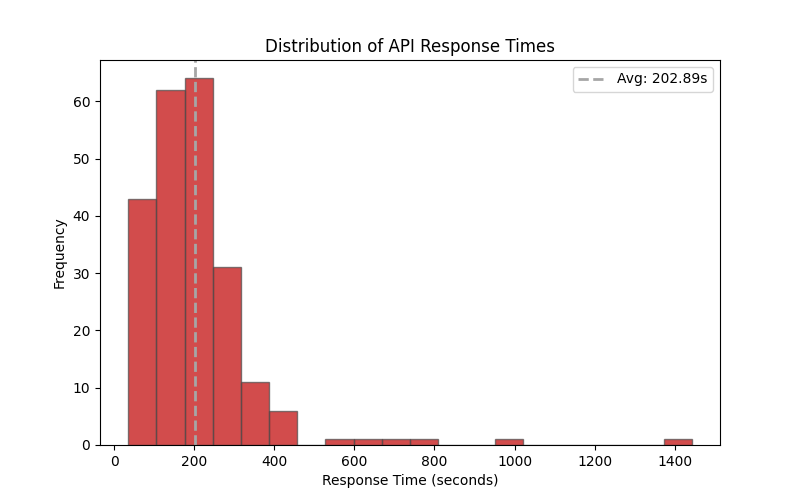
\includegraphics[width=0.8\linewidth]{img/response_time}
    \caption{Average computational time for one query to the LLM. To process 20 thousand documents, 40 thousand queries are required, for a total elaboration time of around 90 days.}
    \label{fig:response_time}
\end{figure}

The proposed methodology demonstrates strong potential when the sentiment index is based on a sufficient number of observations, ensuring that the resulting measure is both stable and representative.
This analysis suggests that in private equity, certain general partners (GPs) appear more consistent in maintaining the expectations they set, while others exhibit greater variability, potentially reflecting differences in communication strategies or internal forecasting accuracy.
However, one critical limitation is computational efficiency: processing large volumes of unstructured text data can become prohibitively time-consuming (see Fig.\ref{fig:response_time} for the average time required to handle just one query) without access to adequate computing resources, especially when applying advanced language models.
Another challenge lies in the heterogeneity of the dataset.
Mixing funds across asset classes and incorporating statements from both GPs and limited partners (LPs) can introduce noise, making it harder to draw clear causal inferences. 
This highlights the importance of segmenting the analysis by fund type, region, or strategy to improve robustness and interpretability.
Despite these limitations, the methodology is highly promising.
It is inherently scalable and can be adapted to a wide range of applications, from monitoring market sentiment in real time to enhancing risk models for capital allocation.
As computational infrastructure improves and more granular data becomes available, this approach could become a standard tool for analyzing belief formation and expectation management in private markets.

\section{Roadmap for Extension}
    Here I present some extensions to overcome the limitations found in my research.

    \paragraph{Deployment on ULHPC and usage of more advanced models} On the local machine, inference was carried out on an NVIDIA GeForce GTX~1070 GPU with 8\,GB of VRAM (CUDA~12.8), which limited the feasible model size and imposed a maximum context length of 2,048 tokens for Deepseek~8B.
    This required documents to be split into multiple segments for processing.
    In contrast, the ULHPC nodes are equipped with NVIDIA Tesla V100-SXM2 GPUs with 32\,GB of VRAM  (CUDA~12.7), offering four times the memory capacity and significantly greater computational capacity.
    This would enable the use of both Deepseek~8B and larger model such as GPT-OSS~20B with extended context lengths of up to 131,072 tokens, allowing entire documents to be processed in a single pass, thereby reducing preprocessing overhead and improving throughput.
    In particular, it would significantly reduce the computational time needed.

    \begin{lstlisting}[style=cmd,label={lst:gptoss}]
        Model
            architecture        gptoss
            parameters          20.9B
            context length      131072
            embedding length    2880
            quantization        MXFP4

        Capabilities
            completion
            tools
            thinking

        Parameters
            temperature    1

        License
            Apache License
            Version 2.0, January 2004
    \end{lstlisting}

    \paragraph{Investigate other quantities and other forecasting horizons} This research was limited to forecasting changes in distribution cashflows in the next year.
    With better hardware and more time to experiment, it will be possible to ask about other quantities, such as returns and fundraising, and different time horizons, such as the next quarter, or the next 2 years.

    \paragraph{Improve Granularity} While the aggregation per GP provides an immediate overview of the performance of its funds, in reality it often aggregates funds from different asset classes (such as Buyout, Venture Capital, Real Estate and Fund of Funds) which often perform in very different ways.
    Moreover, there are other important factors that influence the performances of a fund, for instance the Vintage effect, i.e. the years since its inception which determine at which stage of its life the fund is.
    Therefore, it would be more appropriate to create indices for each fund and then aggregate appropriately per GP or Asset Class.

% ===============================
\appendix